\documentclass[journal,12pt,twocolumn]{IEEEtran}

\usepackage{setspace}
\usepackage{gensymb}

\singlespacing


\usepackage[cmex10]{amsmath}

\usepackage{amsthm}

\usepackage{mathrsfs}
\usepackage{txfonts}
\usepackage{stfloats}
\usepackage{bm}
\usepackage{cite}
\usepackage{cases}
\usepackage{subfig}

\usepackage{longtable}
\usepackage{multirow}

\usepackage{enumitem}
\usepackage{mathtools}
\usepackage{steinmetz}
\usepackage{tikz}
\usepackage{circuitikz}
\usepackage{verbatim}
\usepackage{tfrupee}
\usepackage[breaklinks=true]{hyperref}
\usepackage{graphicx}
\usepackage{tkz-euclide}
\usepackage{float}

\usetikzlibrary{calc,math}
\usepackage{listings}
    \usepackage{color}                                            %%
    \usepackage{array}                                            %%
    \usepackage{longtable}                                        %%
    \usepackage{calc}                                             %%
    \usepackage{multirow}                                         %%
    \usepackage{hhline}                                           %%
    \usepackage{ifthen}                                           %%
    \usepackage{lscape}     
\usepackage{multicol}
\usepackage{chngcntr}

\DeclareMathOperator*{\Res}{Res}

\renewcommand\thesection{\arabic{section}}
\renewcommand\thesubsection{\thesection.\arabic{subsection}}
\renewcommand\thesubsubsection{\thesubsection.\arabic{subsubsection}}

\renewcommand\thesectiondis{\arabic{section}}
\renewcommand\thesubsectiondis{\thesectiondis.\arabic{subsection}}
\renewcommand\thesubsubsectiondis{\thesubsectiondis.\arabic{subsubsection}}


\hyphenation{op-tical net-works semi-conduc-tor}
\def\inputGnumericTable{}                                 %%

\lstset{
%language=C,
frame=single, 
breaklines=true,
columns=fullflexible
}
\begin{document}
\newtheorem{theorem}{Theorem}[section]
\newtheorem{problem}{Problem}
\newtheorem{proposition}{Proposition}[section]
\newtheorem{lemma}{Lemma}[section]
\newtheorem{corollary}[theorem]{Corollary}
\newtheorem{example}{Example}[section]
\newtheorem{definition}[problem]{Definition}

\newcommand{\BEQA}{\begin{eqnarray}}
\newcommand{\EEQA}{\end{eqnarray}}
\newcommand{\define}{\stackrel{\triangle}{=}}
\bibliographystyle{IEEEtran}
\providecommand{\mbf}{\mathbf}
\providecommand{\pr}[1]{\ensuremath{\Pr\left(#1\right)}}
\providecommand{\qfunc}[1]{\ensuremath{Q\left(#1\right)}}
\providecommand{\sbrak}[1]{\ensuremath{{}\left[#1\right]}}
\providecommand{\lsbrak}[1]{\ensuremath{{}\left[#1\right.}}
\providecommand{\rsbrak}[1]{\ensuremath{{}\left.#1\right]}}
\providecommand{\brak}[1]{\ensuremath{\left(#1\right)}}
\providecommand{\lbrak}[1]{\ensuremath{\left(#1\right.}}
\providecommand{\rbrak}[1]{\ensuremath{\left.#1\right)}}
\providecommand{\cbrak}[1]{\ensuremath{\left\{#1\right\}}}
\providecommand{\lcbrak}[1]{\ensuremath{\left\{#1\right.}}
\providecommand{\rcbrak}[1]{\ensuremath{\left.#1\right\}}}
\theoremstyle{remark}
\newtheorem{rem}{Remark}
\newcommand{\sgn}{\mathop{\mathrm{sgn}}}
\providecommand{\abs}[1]{\vert#1\vert}
\providecommand{\res}[1]{\Res\displaylimits_{#1}} 
\providecommand{\norm}[1]{\lVert#1\rVert}
%\providecommand{\norm}[1]{\lVert#1\rVert}
\providecommand{\mtx}[1]{\mathbf{#1}}
\providecommand{\mean}[1]{E[ #1 ]}
\providecommand{\fourier}{\overset{\mathcal{F}}{ \rightleftharpoons}}
%\providecommand{\hilbert}{\overset{\mathcal{H}}{ \rightleftharpoons}}
\providecommand{\system}{\overset{\mathcal{H}}{ \longleftrightarrow}}
	%\newcommand{\solution}[2]{\textbf{Solution:}{#1}}
\newcommand{\solution}{\noindent \textbf{Solution: }}
\newcommand{\cosec}{\,\text{cosec}\,}
\providecommand{\dec}[2]{\ensuremath{\overset{#1}{\underset{#2}{\gtrless}}}}
\newcommand{\myvec}[1]{\ensuremath{\begin{pmatrix}#1\end{pmatrix}}}
\newcommand{\mydet}[1]{\ensuremath{\begin{vmatrix}#1\end{vmatrix}}}
\numberwithin{equation}{subsection}
\makeatletter
\@addtoreset{figure}{problem}
\makeatother
\let\StandardTheFigure\thefigure
\let\vec\mathbf
\renewcommand{\thefigure}{\theproblem}
\def\putbox#1#2#3{\makebox[0in][l]{\makebox[#1][l]{}\raisebox{\baselineskip}[0in][0in]{\raisebox{#2}[0in][0in]{#3}}}}
     \def\rightbox#1{\makebox[0in][r]{#1}}
     \def\centbox#1{\makebox[0in]{#1}}
     \def\topbox#1{\raisebox{-\baselineskip}[0in][0in]{#1}}
     \def\midbox#1{\raisebox{-0.5\baselineskip}[0in][0in]{#1}}
\vspace{3cm}
\title{GATE ASSIGNMENT 4}
\author{Dishank Jain \\ AI20BTECH11011}
\maketitle
\newpage
\bigskip
\renewcommand{\thefigure}{\theenumi}
\renewcommand{\thetable}{\theenumi}
Download latex-tikz codes from
%
\begin{lstlisting}
https://github.com/Dishank422/EE3900/blob/main/Gate-Assignment4/latex_code.tex
\end{lstlisting}
%
\section{EC 1999 Q.2.1}
The Fourier representation of an impulse train represented by $s(t) = \sum_{n=-\infty}^{\infty}\delta(t-nT_0)$ is given by
\begin{enumerate}[label=(\alph*)]
\setlength\itemsep{0.5em}
    \item $\frac{1}{T_0}\sum_{n=-\infty}^{\infty}\exp\brak{-\frac{j2\pi nt}{T_0}}$
    \item $\frac{1}{T_0}\sum_{n=-\infty}^{\infty}\exp\brak{-\frac{j\pi nt}{T_0}}$
    \item $\frac{1}{T_0}\sum_{n=-\infty}^{\infty}\exp\brak{\frac{j\pi nt}{T_0}}$
    \item $\frac{1}{T_0}\sum_{n=-\infty}^{\infty}\exp\brak{\frac{j2\pi nt}{T_0}}$
\end{enumerate}

\section{Solution}
\begin{lemma}
Any periodic signal x(t) with period $T_0$ can be written as 
\begin{equation}
    x(t) = \sum_{n=-\infty}^{\infty} a_n \exp \brak{\dfrac{j2\pi nt}{T_0}}\label{analysis}
\end{equation}
where, $a_n$ is given by
\begin{equation}
    a_n = \dfrac{1}{T_0}\int_{T_0}x(t)\exp\brak{-\dfrac{j2\pi nt}{T_0}}dt\label{synthesis}
\end{equation}
\end{lemma}
\begin{proof}
We shall verify equation \ref{synthesis}. 
\begin{align}
    a_n &= \dfrac{1}{T_0}\int_{T_0}x(t)\exp\brak{-\dfrac{j2\pi nt}{T_0}}dt\\
        &= \dfrac{1}{T_0}\int_{T_0}\brak{\sum_{m=-\infty}^{\infty} a_m \exp \brak{\dfrac{j2\pi mt}{T_0}}}\exp\brak{-\dfrac{j2\pi nt}{T_0}}dt\\
        &= \dfrac{1}{T_0}\sum_{m=-\infty}^{\infty}\int_{T_0}a_m \brak{\exp \dfrac{j2\pi mt}{T_0}}\exp\brak{-\dfrac{j2\pi nt}{T_0}}dt\label{an}
\end{align}
When $m = n$,
\begin{align}
    \int_{T_0}a_m \exp \brak{\dfrac{j2\pi mt}{T_0}}\exp\brak{-\dfrac{j2\pi nt}{T_0}}dt &= \int_{T_0} a_n\\
    &= T_0 a_n
\end{align}
When $m \ne n$,
\begin{align}
    &\int_{T_0}a_m \exp \brak{\dfrac{j2\pi mt}{T_0}}\exp\brak{-\dfrac{j2\pi nt}{T_0}}dt\\ 
    &= a_m\int_{T_0}\exp \brak{\dfrac{j2\pi (m-n)t}{T_0}} dt
\end{align}
Since $\exp \brak{\frac{j2\pi (m-n)t}{T_0}}$ is periodic with period $\frac{T_0}{m-n}$, it's integral over any time interval of length $\frac{T_0}{m-n}$ or any integral multiple of $\frac{T_0}{m-n}$ will be 0. Therefore, when $m \ne n$,
\begin{equation}
    \int_{T_0}a_m \exp \brak{\dfrac{j2\pi mt}{T_0}}\exp\brak{-\dfrac{j2\pi nt}{T_0}}dt = 0
\end{equation}
Continuing from equation \ref{an},
\begin{align}
    a_n &=  \dfrac{1}{T_0}\sum_{m=-\infty}^{\infty}\int_{T_0}a_m \exp \brak{\dfrac{j2\pi mt}{T_0}}\exp\brak{-\dfrac{j2\pi nt}{T_0}}dt\\
    &= \dfrac{1}{T_0}(T_0a_n) = a_n
\end{align}
\end{proof}
We observe that $s(t)$ is periodic with period $T_0$. Thus it's Fourier representation as a sum of complex exponents is given by
\begin{equation}
    s(t) = \sum_{n=-\infty}^{\infty}a_n\exp\brak{\dfrac{j2\pi nt}{T_0}}
\end{equation}
where, $a_n$ can be calculated as
\begin{equation}
    a_n = \dfrac{1}{T_0}\int_{-\frac{T_0}{2}}^{\frac{T_0}{2}}s(t)\exp\brak{-\dfrac{j2\pi nt}{T_0}}dt
\end{equation}
Between $-\dfrac{T_0}{2}$ and $\dfrac{T_0}{2}$, we can say that $s(t) = \delta(t)$.
\begin{align}
    \implies a_n &= \dfrac{1}{T_0}\int_{-\frac{T_0}{2}}^{\frac{T_0}{2}}\delta(t)\exp\brak{-\dfrac{j2\pi nt}{T_0}}dt\\
        &= \dfrac{1}{T_0}\\
    \implies s(t) &= \dfrac{1}{T_0}\sum_{n=-\infty}^{\infty}\exp\brak{\dfrac{j2\pi nt}{T_0}}\label{series}
\end{align}
Therefore option (d) is the correct option.
\begin{lemma}
The Fourier transform of $\exp \brak{j2\pi f_0t}$ is $2\pi \delta(f-f_0)$.
\end{lemma}
\begin{proof}
We verify the lemma by finding the inverse Fourier transform of $2\pi \delta(f-f_0)$.
\begin{align}
    \dfrac{1}{2\pi}\int_{-\infty}^{\infty}2\pi \delta(f-f_0)\exp \brak{j2\pi f t}df = \exp \brak{j2\pi f_0 t}
\end{align}
\end{proof}
Let $S(f)$ be the Fourier transform of s(t). Then using the above lemma and equation \ref{series}
\begin{equation}
    S(f) = \dfrac{2\pi}{T_0}\sum_{n=-\infty}^{\infty}\delta\brak{f-\dfrac{n}{T_0}}
\end{equation}
We can also write the above by substituting $\omega_0 = \dfrac{1}{T_0}$ as
\begin{equation}
    S(f) = \sum_{n=-\infty}^{\infty}2\pi f_0\delta\brak{f-nf_0}
\end{equation}
Thus we can observe that the Fourier transform of an impulse train is an impulse train in the frequency domain.
%\begin{figure}
%    \centering
%    \resizebox{\columnwidth}{!}{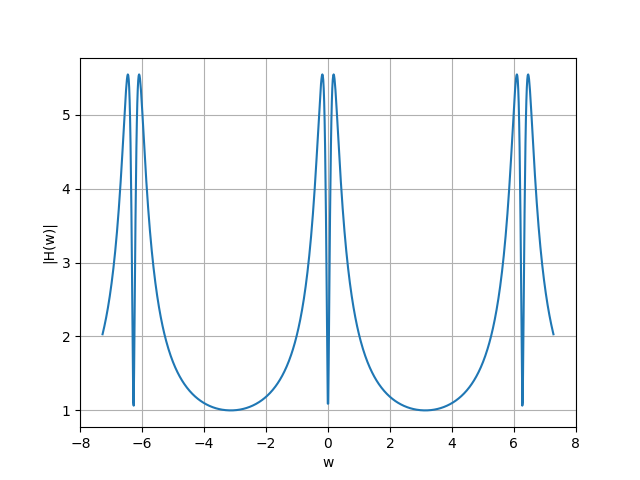
\includegraphics{figures/DTFT.png}}
%    \caption{DTFT of the filter}
%    \label{DTFT}
%\end{figure}
\end{document}
